Particle physics is the branch of physics that studies the fundamental constituents of matter and the forces governing their interactions.  
The field started as studies in electromagnetism, radiation, and further developed with the discovery of the electron.
What followed was more experiments to search for new particles, new models to describe the results, and new search techniques which demanded more data.
The balance in resources for an experiment bottlenecks how much data can be taken, so steps need to be taken to identify interesting interactions and optimize the storage and processing of this data.
This thesis investigates software performance optimization of the ATLAS experiment at CERN. 
Specifically, ways to modernize and optimize areas of the software framework, Athena, to improve input/output (I/O) performance during derivation production and create new tests that catch when specific core I/O functionality is broken.

\section{LHC and The ATLAS Detector}

\begin{figure}[h]
    \centering
    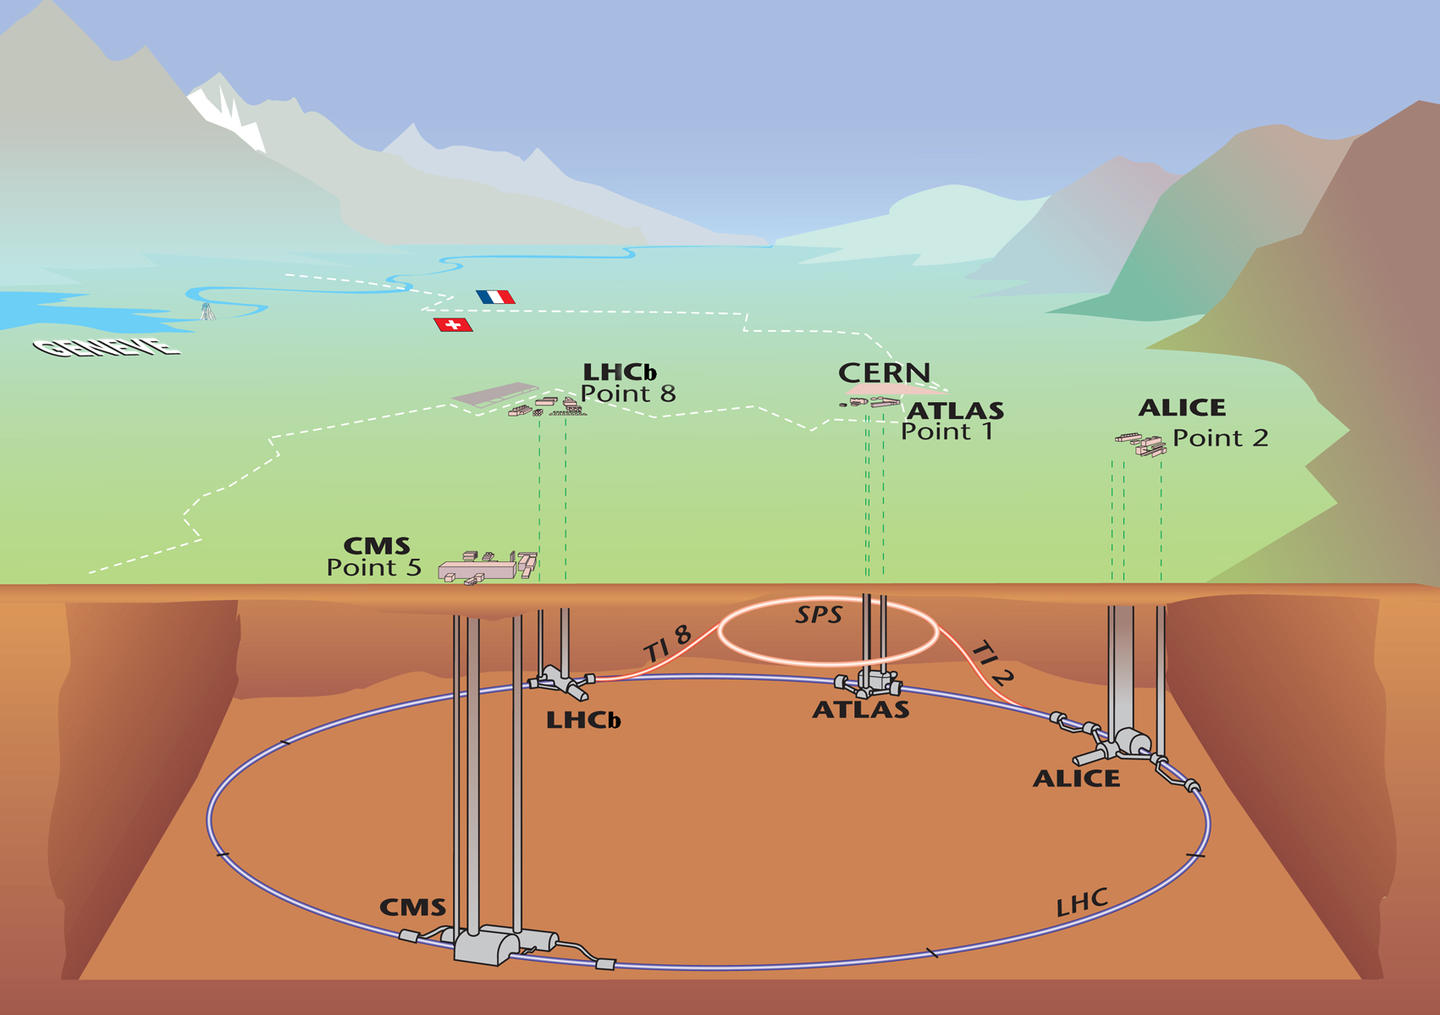
\includegraphics[width=.8\textwidth]{content/img/LHC illustration.jpg}
    \caption{Illustration of the LHC experiment sites on the France-Switzerland border.\cite{LHC_Illustration}}
    \label{fig:intro_LHC_sites}
\end{figure}

The Large Hadron Collider (LHC), shown in Figure \ref{fig:intro_LHC_sites},  is a particle accelerator spanning a 26.7-kilometer ring that crosses between the France-Switzerland border at a depth between 50 and 175 meters underground.\cite{Bruning:782076}
The ATLAS experiment, shown in Figure \ref{fig:intro_ATLAS_detector}, is the largest LHC general purpose detector, and the largest detector ever made for particle collision experiments. 
The detector lies in a cavern 92.5 m underground at a length of 46 m, height and width of 25 m.\cite{ATLAS_Tech_Proposal}
A quadrant of the detector is shown in Figure \ref{fig:ATLAS_quadrant}, where $\eta$ is a measure of the pseudo-rapidity.
Pseudo-rapidity is a parameter representing the the angle relative to the beamline and is defined as
\begin{equation}
    \eta \equiv -\ln\left[ \tan\left(\frac{\theta}{2}\right)\right],
\end{equation}  
where if $\theta = 0$ then $\eta = \infty$ and if $\theta = \frac{\pi}{2}$ then $\eta = 0$.
Pseudo-rapidity is used, as opposed to traditional Cartesian angles, because it's Lorentz invariant under boosts along the beam axis, making it easier to identify tracks due to symmetry of the collision.  
\begin{figure}[h!]
    \centering
    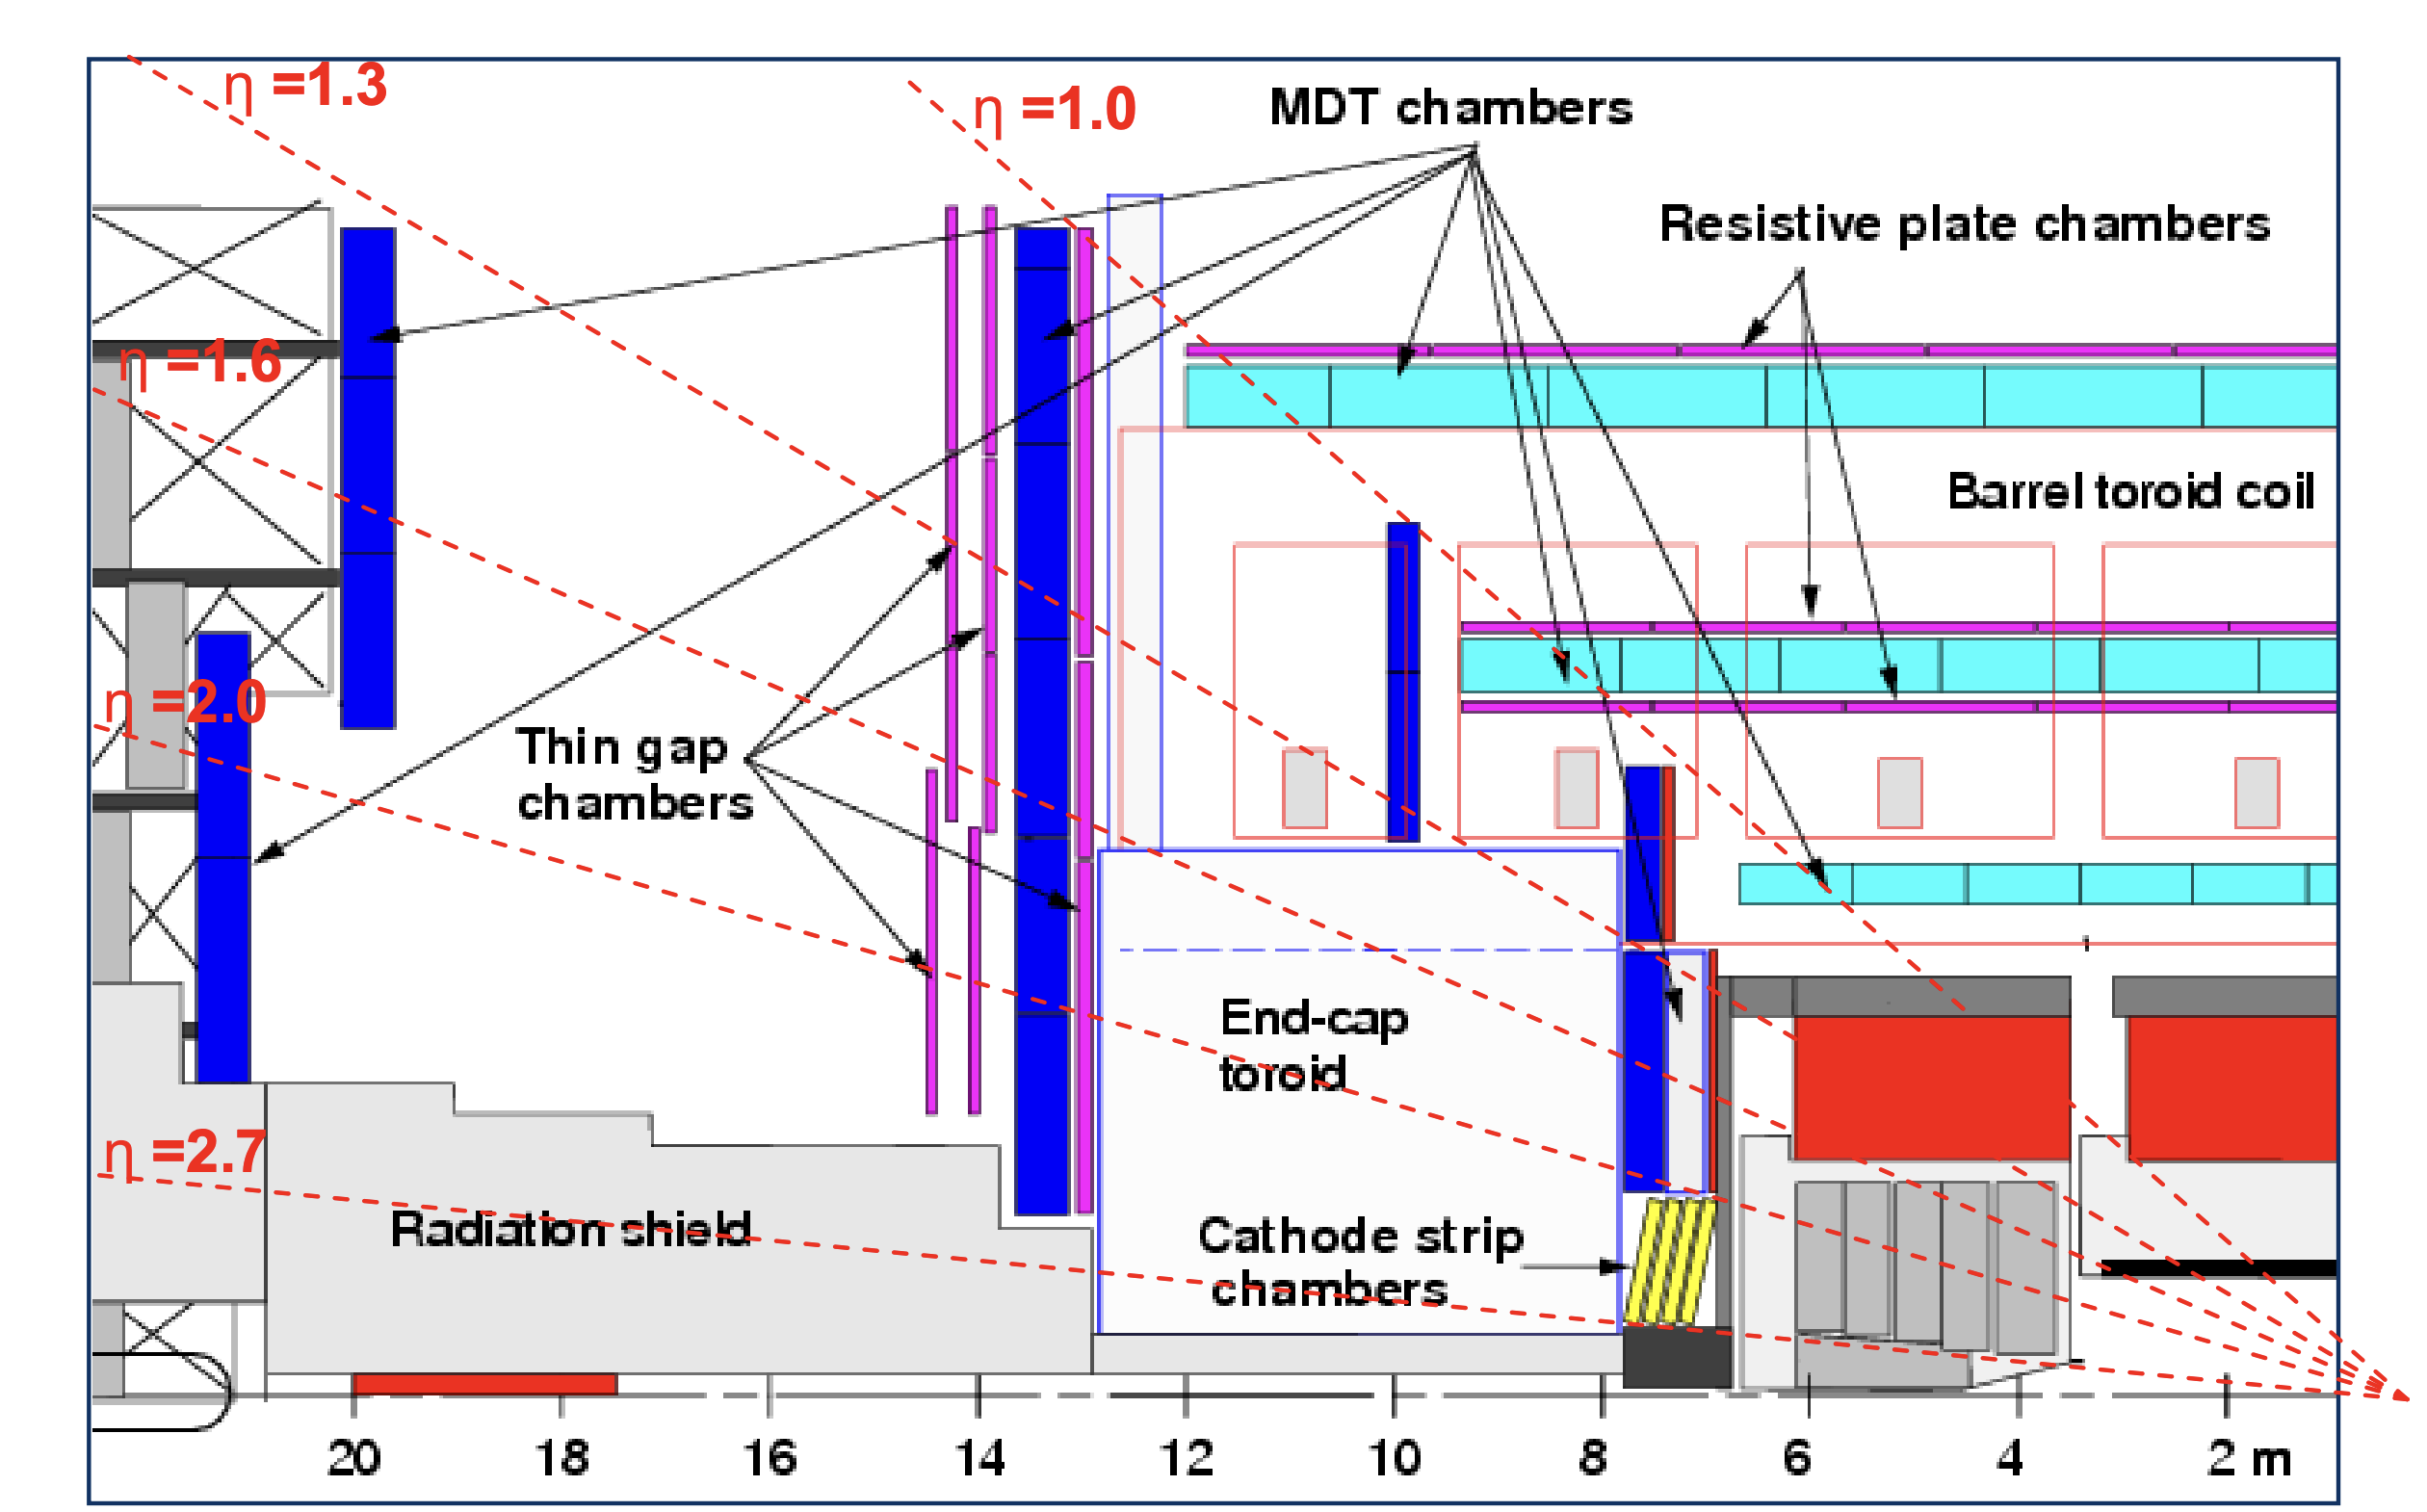
\includegraphics[width=.8\textwidth]{content/img/ATLAS qudrant labelled MS.png}
    \caption{One quadrant of the ATLAS detector. The components of the Muon Spectrometer are labelled \cite{Hough_Transform_CSC}}
    \label{fig:ATLAS_quadrant}
\end{figure}

\begin{figure}[h]
    \centering
    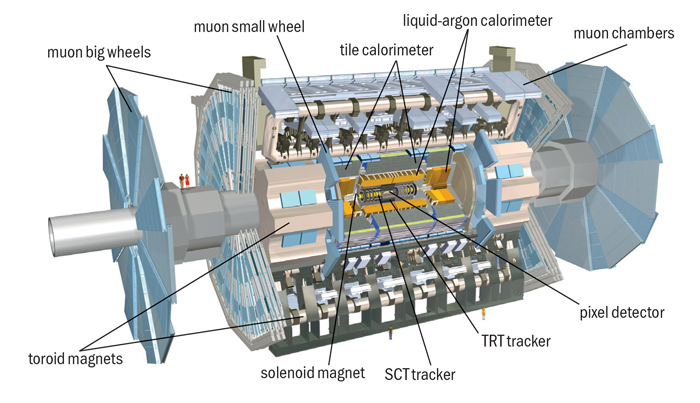
\includegraphics[width=.8\textwidth]{content/img/ATLAS_Detector.jpg}
    \caption{Overview of the ATLAS detectors main components, with two people in figure to scale.\cite{ATLAS_Illustration}}
    \label{fig:intro_ATLAS_detector}
\end{figure}

\noindent\textbf{Inner Detector}

The ATLAS detector is comprised of three main sections, the inner detector, calorimeters and the muon detector system. 
The inner detector measures the direction, momentum and charge of electrically charged particles.
Its main function is to measure the track of the charged particles without destroying the particle itself.
The first point of contact for particles emerging from $pp$-collisions from the center of the ATLAS detector is the pixel detector.\cite{PixelDetector_2008}
It has over 92 million pixels to aid in particle track and vertex reconstruction.
Since the pixels are the first point of contact to the incident particles they have to be radiation hard so the electronics may function without fault.
When a charged particle passes through a pixel sensor it ionizes the one-sided doped-silicon wafer to produce an excited electron will then occupy the conduction band of the semiconductor producing an electron-hole pair, leaving the valence band empty.\cite{KnollRadDetection}
This hole in the valence band together with the excited electron in the conduction band is called an electron-hole pair.
The electron-hole pair is in the presence of an electric field, which will induce drifting of the electron-hole pair, drifting that will generate the electric current to be measured.

Surrounding the pixel detector is the SemiConductor Tracker (SCT), which uses 4,088 modules of 6 million implanted silicon readout strips.\cite{ABDESSELAM2006642}
Both the pixel detector and SCT measure the path particles take, called tracks.
While the pixel detector has measurement precision up to $10 \mu m$ in the $r\phi$-direction and $70 \mu m$ in the $z$-coordinate direction,\cite{Andreazza:1287089} the SCT has resolution $17 \mu m$ in the $r\phi$-direction and $580 \mu m$ in the $z$-direction. 

The final layer of the inner detector is the transition radiation tracker (TRT). 
The TRT is made of a collection of tubes made with many layers of different materials with varying indices of refraction.
The TRT's straw walls are made of two $35\mu m$ layers comprised of $6\mu m$ carbon-polymide, $0.20 \mu m$ aluminum, and a $25\mu m$ Kapton film reflected back.\cite{TRT_2008}
The straws are filled with a gas mixture of $70\% \text{Xe} + 27\% \text{CO}_2 + 3\% \text{O}_2$. 
Its measurement precision is around $170 \mu m$. 
Particles with relativistic velocities have higher Lorentz $\gamma$-factors,
\begin{equation}\label{lorentzGamma}
    \gamma = \frac{1}{\sqrt{1 - \frac{v^2}{c^2}}}.
\end{equation}
The TRT uses varying materials to discriminate between heavier particles, which have low $\gamma$ and radiate less, and lighter particles, which have higher $\gamma$ and radiate more.\cite{Mindur:2139567}

\pagebreak
\noindent\textbf{Calorimeters}

There are two main calorimeters for ATLAS, the Liquid Argon (LAr) calorimeter and the Tile Hadronic calorimeter.
The LAr calorimeter surrounds the inner detector and measures the energy deposits of objects that interact via the electromagnetic force. 
It layers various metals to intercept the incoming particles to produce a shower of lower energy particles. 
The lower energy particles then ionize the liquid argon that fill the barrier in between the metal layers to produce a current that can be read out.
The Tile calorimeter surrounds the LAr calorimeter and is the largest part of the ATLAS detector weighing in around 2900 tons. 
Particles then traverse through the layers of steel and plastic scintillating tiles. 
The Tile calorimeter is a hadronic calorimeter, so it interacts with particles via the strong nuclear force. 
When a particle hits the steel, a cascade of secondary protons, neutrons and other hadrons (quark bound states, with baryons $qqq$ and mesons $q\bar{q}$) is produced with lower energy. 
Through this mechanism, these decay products will continue until the energy has entirely dissipated.

% Discuss the Muon spectrometer
\noindent\textbf{Muon Spectrometer (MS)}

The MS sits at the end of the ATLAS detector and is designed to identify muon tracks and momentum to high-resolution, its components are shown in Figure \ref{fig:ATLAS_quadrant}.
Monitored Drift Tube (MDT) chambers are used for precision measurement of muon tracks in the principle bending direction of the magnetic fields over a large $\eta$.
The MDT lie in the endcaps and barrel regions covering the pseudorapidity regions $0 < |\eta| < 2.7$, where the the tubes run perpendicular to the beam and in-line with the magnetic field lines.
Single cell resolution for these drift tubes can reach $60 \mu m$.\cite{ATLAS_Tech_Proposal}
The area of highest particle flux is the region of pseudo-rapidity $2 < |\eta| < 2.7$, here is where the cathode strip chambers lie.\cite{muonSpec}
Cathode strip chambers (CSCs) are layered to determine track vectors and use multi-wire chambers to achieve a resolution up to $50 \mu m$. 

The RPCs are gaseous parallel-plate detectors suited for fast spacetime particle tracking that combines the the spatial resolution (around 1 cm) of the wire chambers and the time resolution (around 1 ns) of a scintillation counter.
Resistive plate chambers (RPCs) and the Thin gap chambers (TGCs) provide the trigger information for the MDTs and CSCs to then make a precision measurement, so speed takes priority over spatial resolution for the muon trigger system. 
Though RPCs don't have wires, their design consists of two strips separated by an insulating spacer to create a gap for the gas ($C_2 H_2 F_4$ plus some smaller of argon/butane) to occupy.
Thin gap chambers (TGCs) exist in the forward region and are thin wire chambers that aide in muon triggering and measurement of the azimuthal coordinate to be used in compliment with MDTs.
The time resolution in TCGs help identify bunch-crossings and granularity in momentum of the muon that comes within the equipotential of the wires. 
Since each wire can be given a position in the trigger system, any muon that passes through the TGC can be compared with greater spatial precision with the MDTs and illustrate a track later.
The accuracy of identifying the correct bunch crossing with TGCs is 99\% and the delivery of bunch crossing identification can be delivered within 25 ns, only a small fraction of bunch crossings arrive later than that window.

\section{ATLAS Trigger/Data Acquisition (TDAQ)}

The LHC produces $pp$-collisions at a rate of 40 MHz, each collision is an ``event". 
More specifically, around $10^{11}$ protons are accelerated in one ``bunch" with around 2800 bunches per proton beam spaces around 25 ns apart from each other. 
Each beam is then concentrated to the width of $64 \mu m$ at the interaction point where about 20 collisions happen at one bunch crossing, these collisions within one bunch results in ``pile-up".

% What is the ATLAS Trigger System
The ATLAS Trigger system is responsible for quickly deciding what events are interesting for physics analysis.
The Trigger system is divided into the first- and second-level triggers and when a particle activates a trigger, the trigger makes a decision to tell the DAQ to save the data produced by the detector. 
The first-level trigger is a hardware trigger that decides, within $2.5 \mu s$ after the event, if it's a good event to put into a storage buffer for the second-level trigger.
The second-level trigger is a software trigger that decides within $200 \mu s$ and uses around 40,000 CPU-cores and analyses the event to decide if it is worth keeping. 
The second-level trigger selects about 1000 events per second to keep and store long-term.\cite{Trigger-DAQ}
The data taken by the TDAQ system is raw and not yet in a state that is ready for analysis, but it is ready for further processing. 

% Lots of data -> WLCG handles it
The amount of data taken at ATLAS is substantial, seeing more than 3 PB of raw data each year and each individual event being around 2 MB.\cite{ATLAS_Fact_Sheet} 
All of the data produced by LHC experiments, especially ATLAS, has to be sent to the Worldwide LHC Computing Grid (WLCG).\cite{WLCG_Tech_design_report}
% How is it sent to the Grid: Tier 0, 1, 2 sites
The WLCG composes of a three-tiered system, CERN serves as the Tier-0 site, there are $\mathcal{O}(20)$ Tier-1 sites, and $\mathcal{O}(200)$ Tier-2 sites.\cite{Martelli_2015}
Though, the numbers of each site do change over time.
The raw data coming from the TDAQ systems are recorded at the CERN Tier-0 sites where a first-pass at reconstruction will take place and a copy of the raw data is sent to the Tier-1 sites.
Multiple 10 Gbps capacity links streamline dataflow from the ATLAS TDAQ to the Tier-0 site. 
Tier-1 sites offer manage permanent storage of raw and reconstructed data and provide extensive processing capability for analysis that might demand it.
Tier-2 sites provide additional computation and storage services that compliment end-user analysis.

% WLCG handles it -> in what way is it being handled?
Athena manages ATLAS production workflows which are involved with simulation of data and event generation, track reconstruction from hits, and derivation production.\cite{athenadocs}
Figure \ref{fig:ATLAS_data_chain} illustrates the broadstrokes of the entire ATLAS data processing chain for both real detector data and Monte Carlo (MC) simulations. 
MC simulation starts with the event generation (EVNT), following simulation of events hitting the detector (HITS) and further simulation of what would be readout of the detector (RDO).
The reconstructed Analysis Object Data (AOD) are then processed through derivation production jobs that reduces AODs from  $\mathcal{O}(1)$ MB per event to $\mathcal{O}(10)$ kB per event, creating Derived AOD (DAOD). 
Further discussion on the production of DAOD can be found in Section \ref{section: ATLASIO_Derivation}.
\begin{figure}[ht]
    \centering
    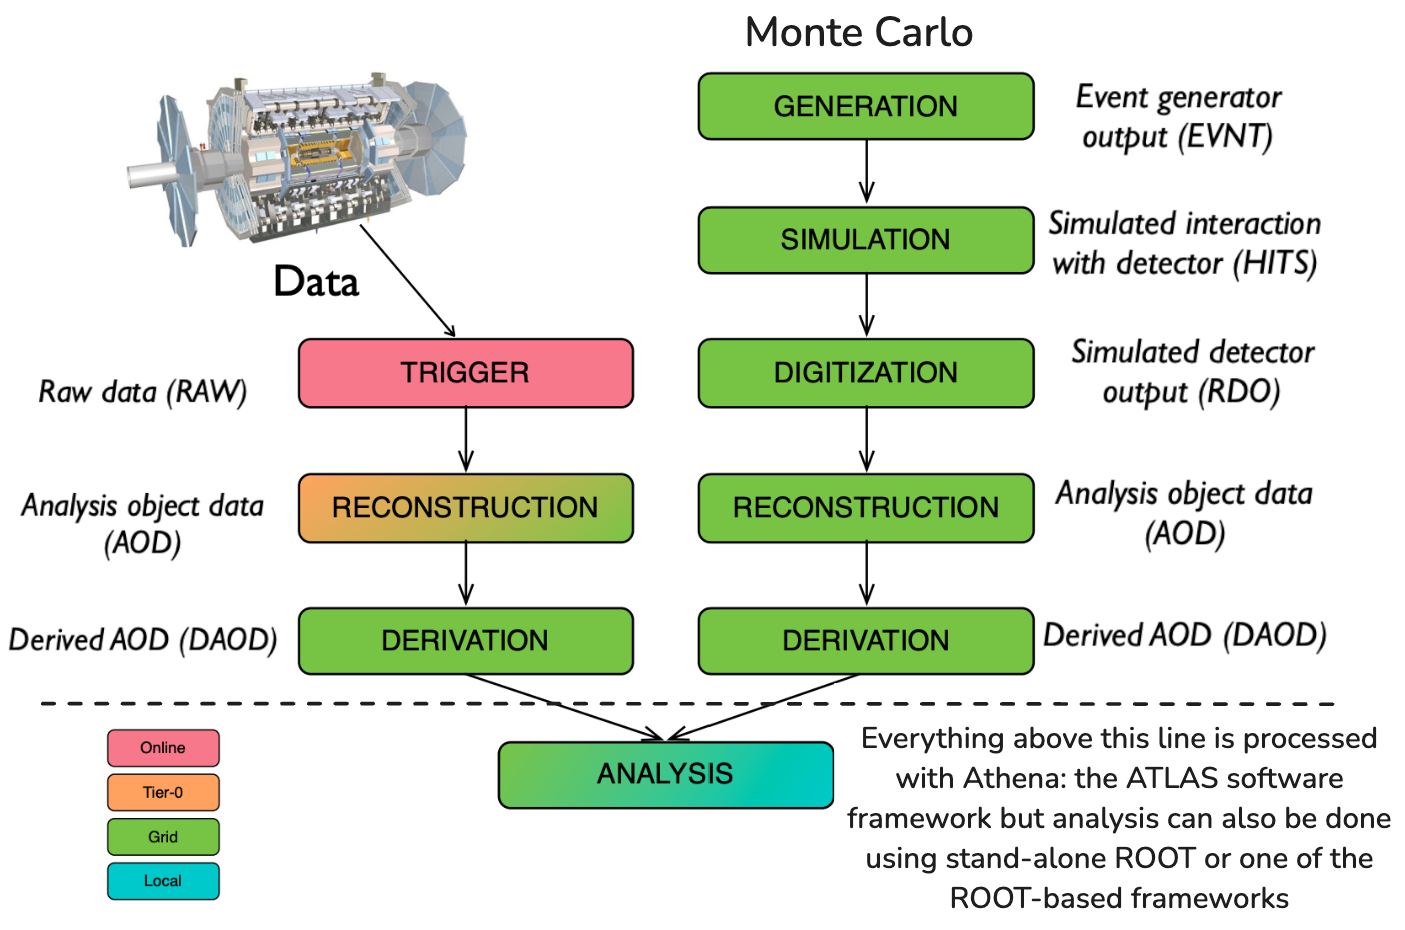
\includegraphics[width=\textwidth]{content/img/modified-James-chain-processing.png}
    \caption{ATLAS data chain-processing for data and Monte Carlo simulation. Figure is modified from \cite{James_Catmore_chain_processing}.}
    \label{fig:ATLAS_data_chain}
\end{figure}



\section{ATLAS Software and Computing Needs}
The High-Luminosity LHC (HL-LHC) is the upgrade to LHC that anticipates more events and more data taken than ever before.
% How does high luminosity affect the number of collisions? 
The goal is to reach a luminosity of $350 fb^{-1}$, which is forecasted to be reached gradually by around 2040.\cite{HL-LHC_Tech_design}
The HL-LHC era is projected to demand anywhere from 6-10 times data stored per year, so any attempt to save on disk storage will help.\cite{ATLAS_HL-LHC_projections}
Increasing data means more resources from the Grid will be needed, so optimization across files and software is an essential part of ensuring scalability of the data taken in by the detector.

The traditional method of storing information for AOD/DAOD is in with ROOT TTrees.




One area of research to account for this flood of new data is in the development of the ROOT N-Tuple (RNTuple) I/O subsystem, which is a new storage format for high-energy physics data seeking to replace ROOT TTree. 
The RNTuple is a columnar-based storage format that is optimized for data storage and processing.
It's been shown to outperform TTree I/O subsystem and other storage formats in file size (by about 15\%), throughput, and compression, but still has more development before full implementation into the analysis pipeline.\cite{RNTuple_Lopez-Gomez_2023}\cite{RNTuple_Blomer}
Additionally, there's a push to utilize GPUs and other accelerators in conjunction with CPUs to process track reconstruction and AOD derivation.
Also being developed are software framework updates, such as AthenaMT, to make the single-threaded CPU programs multi-thread ready.\cite{AthenaMT_Leggett_2017}

